\documentclass{article}

\usepackage{libertine}
\usepackage[libertine]{newtxmath}

\usepackage{hyperref, amsmath, amssymb}
\usepackage{amsfonts}
\usepackage{graphics}
\usepackage{tikz}
\usepackage{graphicx}
\usepackage{enumerate}
\usepackage{color}
\usepackage{mathtools}
\usepackage{stmaryrd}

\usepackage{pgf, latexsym, float, soul, array, booktabs, dsfont, gensymb, wasysym, multicol, tcolorbox, tabularx, enumitem, multirow, vwcol, lipsum}

\usepackage{ marvosym }

\usepackage{enumitem}
\setlist[itemize]{leftmargin=2em, itemsep=-.25em, topsep=0em}

\newenvironment{bx}[1][]{
\begin{tcolorbox}[colback=white!97!black, title=#1, arc=0in, halign=flush left, left=1mm, right=1mm,]
}{
\end{tcolorbox}
}

\DeclareMathOperator{\arcsec}{arcsec}
\DeclareMathOperator{\arccot}{arccot}
\DeclareMathOperator{\arccsc}{arccsc}


\usepackage[margin=0.2in]{geometry}

% \setlength{\columnsep}{1pt}
% \setlength{\columnseprule}{1pt}

\begin{document}
% \begin{huge}
% \begin{center}
% Condensed Calculus
% \end{center}
% \end{huge}
% \noindent \hrule

\begin{center}
\setlength{\tabcolsep}{2pt}
\begin{tabular}{p{2.5in} p{5.25in}}

\begin{bx}[Trigonometry]
$(\cos\theta,\sin\theta)$ is the coordinate on the unit circle that makes angle $\theta$ with the positive $x$-axis.
$$\sec\theta=\frac{1}{\cos\theta}\quad \quad\csc\theta=\frac{1}{\sin\theta}$$
$$\tan\theta=\frac{\sin\theta}{\cos\theta}\quad \quad \cot\theta=\frac{\cos\theta}{\sin\theta}$$
$${\text{Pythagorean}\atop\text{identities}}\begin{cases}
\sin^2\theta + \cos^2\theta = 1 \\
\tan^2\theta + 1 = \sec^2\theta \\
1 + \cot^2\theta = \csc^2\theta
\end{cases}$$
$$\sin(A\pm B)=\sin A\cos B\pm\cos A\sin B$$
$$\cos(A\pm B)=\cos A\cos B\mp\sin A\sin B$$
$$\sin(2\theta)=2\sin\theta\cos\theta$$
$$\cos(2\theta) =\cos^2\theta-\sin^2\theta$$

\begin{center}
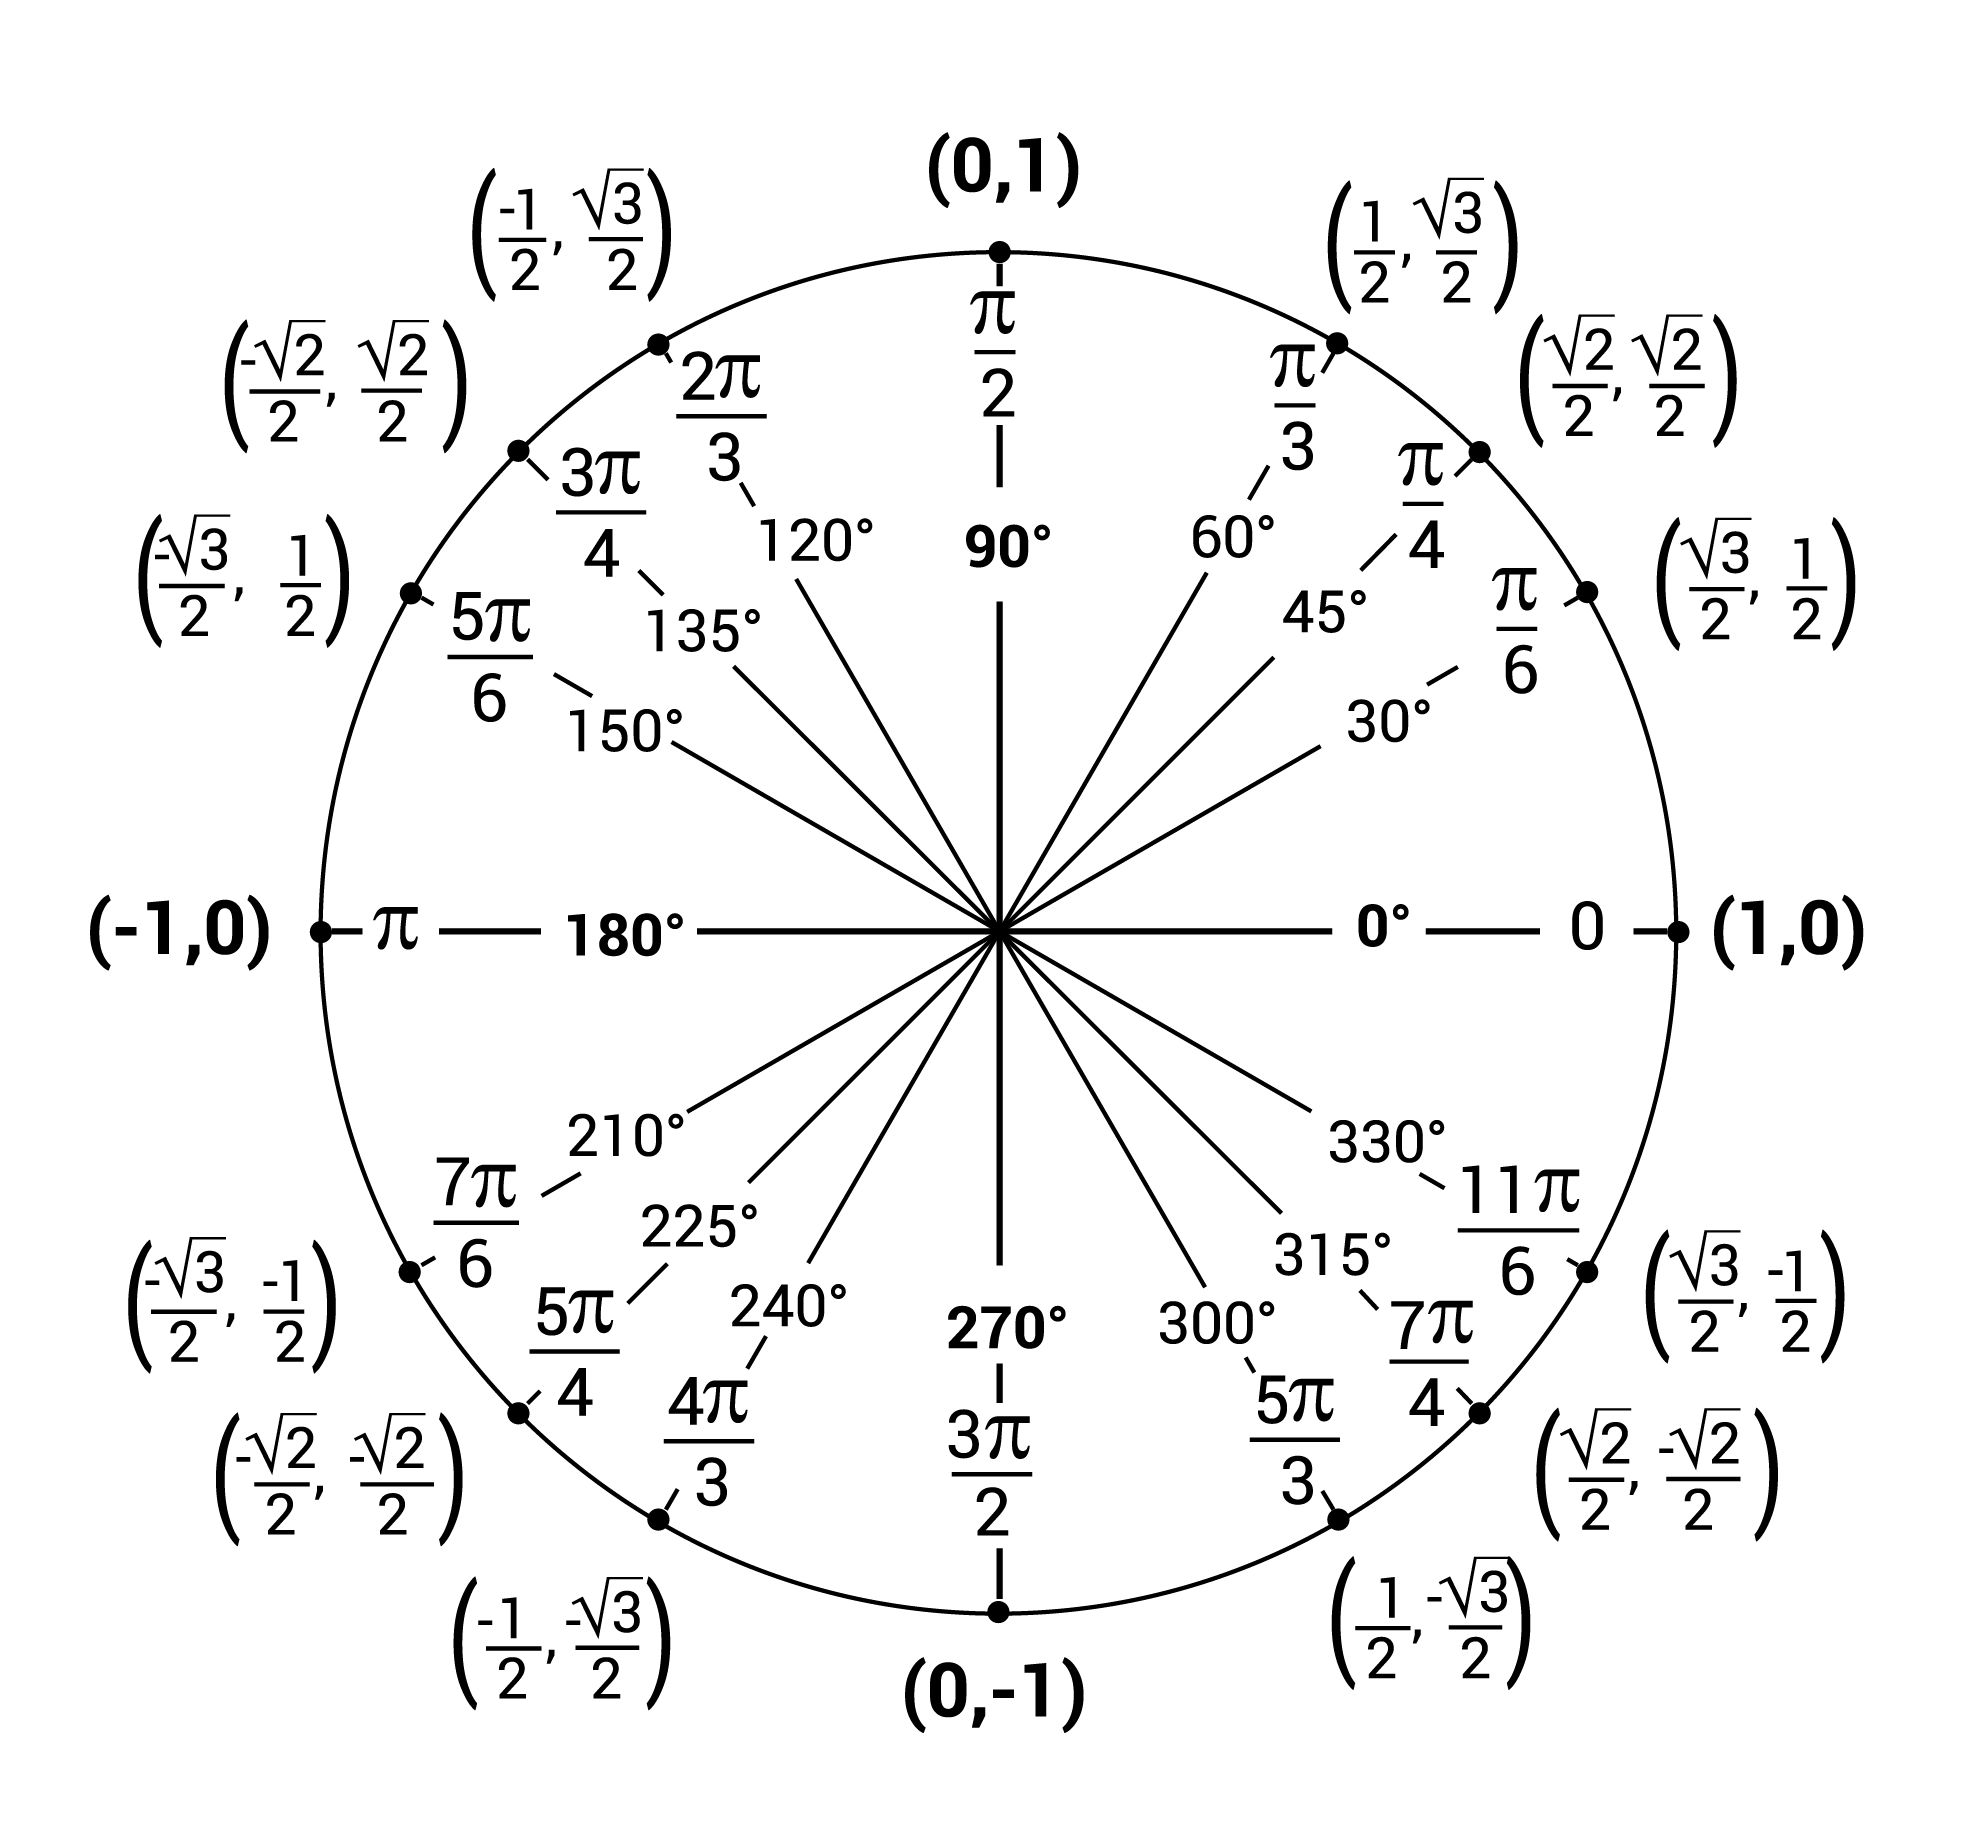
\includegraphics[width=2.3in]{img/unit-circle.png}
\end{center}
\end{bx}

&

\vspace{-5.8in}

\begin{bx}[Limits]
\begin{tabular}{p{3in} p{1.9in}}
\begin{center}

\vspace{-2em}

\def\arraystretch{1.6}
\begin{tabular}{ll}
\textbf{Law} & Let $\displaystyle \lim_{x\to a} f(x)= L$ and $\displaystyle \lim_{x\to a} g(x)= M$.\\
\toprule[0.4mm]
\textbf{Sum} & $\displaystyle\lim _{x \rightarrow a}(f(x)+g(x))=L+M$ \\
\textbf{Scalar} & $\displaystyle\lim _{x \rightarrow a} c f(x)=c L$ \\
\textbf{Product} & $\displaystyle\lim _{x \rightarrow a}(f(x) \cdot g(x))=L \cdot M$ \\
\textbf{Quotient} & $\displaystyle\lim _{x \rightarrow a} \frac{f(x)}{g(x)}=\frac{L}{M}$ for $M \neq 0$ \\
\textbf{Power} & $\displaystyle\lim _{x \rightarrow a}(f(x))^{n}=L^{n}$\\
\textbf{Root} & $\displaystyle\lim _{x \rightarrow a} \sqrt[n]{f(x)}=\sqrt[n]{L}$ for all $L$ if $n$ is odd, \\ & and for $L \geq 0$ if $n$ is even and $f(x) \geq 0 .$ \\
\bottomrule[0.4mm]
\end{tabular}
\end{center}
 &
\textbf{Squeeze Theorem:}

Let $f$, $g$, and $h$ be functions with $g(x)\leq f(x)\leq h(x)$ for all $x$ and $\displaystyle\lim_{x\to a}g(x)=L=\lim_{x\to a} h(x)$, then $\displaystyle\lim_{x\to a} f(x)=L$.

\vspace{1em}

\textbf{Indeterminate Forms:}

$\frac{0}{0}$, $\frac{\infty}{\infty}$, $0^0$, $\infty-\infty$, $1^\infty$, $0\cdot\infty$, $\infty^0$

\vspace{1em}

\textbf{$\varepsilon-\delta$ definition:}

$L$ is the limit of $f$ as $x$ approaches $a$ if for all $\varepsilon > 0$, there is some

$\delta > 0$, such that 

$|x - a| < \delta \implies |f(x) - L| <\varepsilon$.

\end{tabular}

\vspace{-0.25em}

$$\lim_{x\to 0}\frac{\sin(x)}{x} = 1\quad\quad\lim_{x\to\infty}\left(1+\frac{1}{x}\right)^x = e\quad\quad \lim_{x\to\infty}\frac{ax^n+\dots}{bx^m+\dots}=\begin{cases}0 & m>n \\ \infty & n > m \\ a/b & n=m\end{cases}$$

\end{bx}

\vspace{-0.8em}

\begin{bx}[Continuity]
\textbf{Definition:} $f$ is \textit{continuous} at $x=a$ if $\displaystyle\lim_{x\to a}f(x)=f(a)$.

\begin{itemize}
\setlength\itemsep{-0.25em}
\item The following functions are \textbf{continuous on their domains}: polynomials, rational functions, trig and inverse trig functions, exponential functions, logarithms.
\item The sum, product, and composition of continuous functions is continuous.
\end{itemize}

\vspace{0.5em}

\begin{tabular}{p{1.9in} | p{3in}}
\textbf{Composite Function Theorem:}

If $f(x)$ is continuous at $L$

and $\displaystyle\lim _{x \to a} g(x)=L$, then

$\displaystyle\lim_{x \to a} f(g(x))=f(L).$
&
\textbf{Intermediate Value Theorem:}

Let $f$ be continuous over a closed, bounded interval $[a, b]$. If $z$ is any real number between $f(a)$ and $f(b)$, then there is a number $c$ in $[a, b]$ satisfying $f(c)=z$.
\end{tabular}

\end{bx}

\end{tabular}

\vspace{-0.8em}

\begin{tabular}{p{563pt}}
\begin{bx}[Finding Derivatives]

\begin{tabular}{p{3in} p{4.4in}}

\textbf{Limit definition} of the derivative:
$$f'(x)=\lim_{h\to 0}\frac{f(x+h)-f(x)}{h}=\lim_{x\to a}\frac{f(x)-f(a)}{x-a}$$
\textbf{Tangent line} to $f(x)$ at $x=a$:
$$L(x)=f(a) + f'(a)(x-a)$$

\textbf{L'H\^opital's Rule:}

If $\displaystyle \lim_{x\to a} f(x)= \lim_{x\to a} g(x)= 0$ or $\infty$, then
$$\lim_{x\to a}\frac{f(x)}{g(x)}=\lim_{x\to a}\frac{f'(x)}{g'(x)}.$$

\vspace{0.25em}

\begin{center}
\def\arraystretch{1.5}
\begin{tabular}{ll}
\toprule[0.4mm]
\textbf{Scalar Rule} & $[af]' = af'$ \\
\textbf{Sum Rule} & $[f + g]' = f' + g'$ \\
\textbf{Product Rule} & $[fg]' = f'g + fg'$ \\
\textbf{Quotient Rule} & $\left[\frac{f}{g}\right]' = \frac{f'g - fg'}{g^2}$ \\
\textbf{Chain Rule} & $[f(g(x))]' = f'(g(x))g'(x)$ \\
\textbf{Inverse Rule} & $[f^{-1}(x)]' = \frac{1}{f'(f^{-1}(x))}$ \\
\bottomrule[0.4mm]
\end{tabular}
\end{center}

&

% \vspace{2em}

\textbf{Logarithmic Differentiation:}

To find the derivative of $y=f(x)^{g(x)}$, take $\ln()$ of both sides, bring $g(x)$ down using the log rule ($\ln(a^b)=b\ln(a)$):
$$\ln(y)=\ln(f(x)^{g(x)})=g(x)\ln(f(x))$$
Then implicitly differentiate and solve for $y'$:
$$y'=f(x)^{g(x)}\left(g'(x)\ln(f(x))+g(x)\frac{f'(x)}{f(x)}\right).$$


\begin{center}
\def\arraystretch{1.5}
\begin{tabular}{lll}
\toprule[0.4mm]
\textbf{Power Rule}        & $[x^a]' = ax^{a-1}$ \\
\textbf{Trig Rules}  & $[\sin(x)]' = \cos(x)$ & $[\cos(x)]' = -\sin(x)$ \\
(PSST!)& $[\tan(x)]'=\sec^2(x)$ & $[\cot(x)]'=-\csc^2(x)$\\
& $[\sec(x)]'=\sec(x)\tan(x)$ & $[\csc(x)]'=-\csc(x)\cot(x)$ \\
\textbf{Inverse Trig Rules} & $[\arcsin(x)]'=\frac{1}{\sqrt{1-x^2}}$ & $[\arccos(x)]'=\frac{-1}{\sqrt{1-x^2}}$\\
& $[\arctan(x)]'=\frac{1}{1+x^2}$ & $[\arccot(x)]'=\frac{-1}{1+x^2}$\\
& $[\arcsec(x)]'=\frac{1}{|x|\sqrt{x^2-1}}$ &
$[\arccsc(x)]'=\frac{-1}{|x|\sqrt{x^2-1}}$  \\
\textbf{Exponent Rule} & $[a^x]' = \ln(a)a^x$ \\
\textbf{Logarithm Rule} & $[\log_a(x)]' = \frac{1}{x\ln(a)}$ \\
\bottomrule[0.4mm]
\end{tabular}
\end{center}

\end{tabular}


\end{bx}
\end{tabular}


\end{center}

\newpage


\begin{bx}[Integration]
\begin{tabular}{p{4in}p{3.5in}}
\textbf{Definitions}
\begin{itemize}[leftmargin=1em]
    \item The \textit{definite integral} of $f$ on $(a,b)$ is written $\int_a^bf(x)\ dx$ and is defined to be the \textit{signed} area between the graph of $f$ and the $x$-axis (if such a quantity exists).
    \item The \textit{indefinite integral} (or \textit{anti-derivative}) of $f$ on is written $\int f(x)\ dx$ or $\int f$ is the family of functions whose derivative is $f$.
\end{itemize}

\vspace{0.5em}

\textbf{Fundamental Theorem of Calculus} If $F'=f$,
    $$\int_a^bf(x)\ dx = F(b)-F(a).$$


& 
\vspace{-2em}

\begin{center}
\def\arraystretch{1.5}
\begin{tabular}{@{}ll@{}}
\toprule[0.4mm]
\textbf{Scalar Rule} & $\int a f = a \int f$. \\
\textbf{Sum Rule} & $\int f + \int g= \int f + \int g$ \\
\textbf{Int. by Parts}
 & $\int f'g = fg - \int fg' $ \\
\textbf{$u$-substitution} & $\int f'(g(x))g'(x)\ dx =  f(g(x))$ \\
\midrule
\textbf{Power Rule}
 & $\displaystyle\int x^a \ dx = \begin{cases}
\frac{1}{a+1}x^{a+1} + C & a \neq -1\\
\ln|x| + C & a = -1
\end{cases}$ \\
\textbf{Trig Rules}  
& $\int \sin(x)\ dx = -\cos(x)+C$\\
& $\int \cos(x)\ dx = \sin(x)+C$ \\

\textbf{Exp. Rules} & $\int a^x\ dx = \frac{1}{\ln(a)}a^x+C$ \\
\bottomrule[0.4mm]
\end{tabular}
\end{center}
\\ 

\end{tabular}

\begin{tabular}{p{3.25in}p{2in}p{1in}}

\def\arraystretch{1.5}
\begin{tabular}{@{}ll@{}}
\multicolumn{2}{l}{\textbf{Partial Fractions}} \\
\toprule[0.4mm]
      Factor & Term in decomposition\\
      \hline
      $ax+b$          & $\frac{A}{ax+b}$ \\
      $(ax+b)^k$      & $\frac{A_1}{ax+b}+\frac{A_2}{(ax+b)^2}+\dots+\frac{A_k}{(ax+b)^k}$ \\
      $ax^2+bx+c$     & $\frac{Ax+B}{ax^2+bx+c}$\\
      $(ax^2+bx+c)^k$ & $\frac{A_1x+B_1}{ax^2+bx+c}+\frac{A_2x+B_2}{(ax^2+bx+c)^2}+\dots+\frac{A_kx+B_k}{(ax^2+bx+c)^k}$ \\
\bottomrule[0.4mm]
\end{tabular}

& 

\def\arraystretch{1.5}
\begin{tabular}{@{}lll@{}}
	\multicolumn{3}{l}{\textbf{Trig Substitutions}} \\
    \toprule[0.4mm]
    Integrand & Substitution & Result \\
    \hline
    $\sqrt{a^2-x^2}$ & $x=a\sin\theta$ & $a\cos\theta$ \\
    $\sqrt{a^2+x^2}$ & $x=a\tan\theta$ & $a\sec\theta$ \\
    $\sqrt{x^2-a^2}$ & $x=a\sec\theta$ & $a\tan\theta$ \\
    \bottomrule[0.4mm]
    \\
\end{tabular}

&

\def\arraystretch{1.5}
\begin{tabular}{@{}l@{}}
\textbf{Other Antiderivatives} \\
 \toprule[0.4mm]
 $\int\ln(x)\ dx = x\ln(x) - x + C$\\
 $\int \tan(x)\ dx = \ln|\cos(x)|+C$ \\
$\int \sec(x)\ dx = \ln|\sec(x)+\tan(x)|+C$\\
 $\int \csc(x)\ dx = \ln|\csc(x)-\cot(x)|+C$ \\
$\int \cot(x)\ dx = \ln|\sin(x)|+C$  \\
    \bottomrule[0.4mm]
\end{tabular}


\end{tabular}
\end{bx}






\begin{multicols}{2}

\begin{bx}[Riemann Sums]
\begin{tabular}{p{155pt} | p{100pt}}
    $ R_n=\sum_{k=1}^{n}f\left(a+k\frac{b-a}{n}\right)\frac{b-a}{n}$ 

$ L_n=\sum_{k=1}^{n}f\left(a+(k-1)\frac{b-a}{n}\right)\frac{b-a}{n}$ 

$ T_n=\sum_{i=k}^{n}\frac{f\left(a+(k-1)\frac{b-a}{n}\right)+f\left(a+k\frac{b-a}{n}\right)}{2}\frac{b-a}{n}$

\vspace{-1em}

$$\lim_{n\to\infty}R_n,L_n,T_n=\int_a^bf(x)\ dx$$

& 
\textbf{Sums of Powers}

\begin{itemize}[leftmargin=0.75em]
    \item $\sum_{k=1}^n 1 = n $
    \item $\sum_{k=1}^n k = \frac{n(n+1)}{2}$
    \item $\sum_{k=1}^n k^2 = \frac{n(n+1)(2n+1)}{6}$
    \item $\sum_{k=1}^n k^3 = \frac{n^2(n+1)^2}{4}$
\end{itemize}
\end{tabular}

\end{bx}


\begin{bx}[Bounds]

If $f(x)>0$ is CTS and decreasing $[1,\infty)$ with $f(n)=a_n$, then for any $N$,
$$\left(\sum_{n=1}^N a_n+\int_{N+1}^\infty f(x)\ dx \right)
\leq \sum_{n=1}^\infty a_n \leq 
\left(\sum_{n=1}^N a_n+  \int_{N}^\infty f(x)\ dx\right).$$

\hrule
\vspace{1em}

Suppose $S=\sum_{n=1}^\infty b_n (-1)^n$ where $b_n\geq 0$, and $b_n$ decreases to 0. Then for any $N$,
$$\left|S-S_N\right|\leq b_{N+1}$$
where $S_N=\sum_{n=1}^N b_n (-1)^n$.
\vspace{1em}

\hrule
\vspace{1em}

\textbf{Taylor's Inequality:}
If for all $x\in [a-d,a+d]$,
$$\left|f^{(k+1)}(x)\right|\leq M,$$
then for all $x\in [a-d,a+d]$,
$$|f(x)-T_k(x)|\leq \frac{M}{(k+1)!}|x-a|^{k+1}.$$




\end{bx}

\columnbreak



\begin{bx}[Test for Convergence and Divergence]

\begin{itemize}[leftmargin=1em]

\item \textbf{Divergence Test:} ${\displaystyle \lim_{n\to\infty}a_n\neq 0 }\implies \sum a_n $ diverges.\\

\item \textbf{Integral Test:}
If $f(x) > 0$ is CTS and decreasing on $[k,\infty)$, and $f(n)=a_n$,
$$\int_k^\infty f(x)\ dx\text{ converges} \iff \sum_{n=k}^\infty a_n\text{ converges}.$$

\item \textbf{The $p$-series Test:}
 If $k>0$, $\displaystyle\sum_{n=k}^\infty\frac{1}{n^p}$ converges $\iff p>1$.


\item \textbf{Comparison Test:}
 If $0\leq a_n\leq b_n$ for all $n$, then
 $$\sum b_n\text{ converges}\implies \sum a_n\text{ converges}.$$


\item \textbf{Limit Comparison Test:}
If $a_n\geq 0$ and $b_n > 0$ for all $n$ and $\displaystyle\lim_{n\to\infty}{a_n}/{b_n}$ is positive and finite, then 
$$\sum a_n\text{ converges }\iff \sum b_n\text{ converges}.$$


\item \textbf{Alternating Series Test:}
If $b_{n} \geq 0$ decreases to 0, $\sum b_{n}(-1)^{n}$ converges.


\item \textbf{Absolute Convergence Test:}
$$\sum |a_n| \text{ converges}\implies \sum a_n\text{ converges}.$$

\item \textbf{Ratio Test:} Define $\displaystyle L= \lim _{n \to \infty}} \left|{a_{n+1}}/{a_{n}}\right|$.\\ If $L<1$, $\sum a_{n}$ converges. If $L>1$,  $\sum a_{n}$ diverges.


\item \textbf{Root Test}
Define $L={\displaystyle\lim _{n \to \infty}}\left|a_{n}\right|^{{1}/{n}}$. If $L<1$, $\sum a_{n}$ converges.\\ If $L>1$,  $\sum a_{n}$ diverges.

\end{itemize}
\end{bx}


\newpage
\begin{bx}[Power Series]
$$\sum_{n=0}^\infty a_n(x-c)^n$$
converges on
$$|x-c|<\lim\left|\frac{a_{n}}{a_{n+1}}\right|.$$
Test the interval's endpoints separately. On some interval centered at $a$,
$$f(x)=\sum_{n=0}^\infty \frac{f^{(n)}(a)}{n!}(x-a)^n.$$
Near $x=a$, 
$$f(x)\approx T_k(x)=\sum_{n=0}^k \frac{f^{(n)}(a)}{n!}(x-a)^n.$$

\begin{center}
\def\arraystretch{1.2}
\begin{tabular}{llc}
\multicolumn{3}{c}{\textbf{Common Taylor Series}}\\
\midrule[0.4mm]
Function & Taylor Series & Interval of Convergence\\
\midrule\\
$e^x$ & \displaystyle\sum_{n=0}^\infty\frac{1}{n!} x^n$ & $\mathbb{R}$ \\\\
$\sin(x)$ & \displaystyle\sum_{n=0}^\infty\frac{(-1)^n}{(2n+1)!}x^{2n+1}$ & $\mathbb{R}$ \\\\
$\cos(x)$ & \displaystyle\sum_{n=0}^\infty\frac{(-1)^n}{(2n)!}x^{2n}$ & $\mathbb{R}$ \\\\
$\frac{1}{1-x}$ & \displaystyle\sum_{n=0}^\infty x^n$ & $(-1,1)$ \\\\
$\ln(1-x)$ & \displaystyle\sum_{n=1}^\infty \frac{-1}{n}x^{n}$ & $[-1,1)$ \\\\
$(x+1)^k$ & \displaystyle\sum_{n=0}^\infty{k\choose n}x^{n}$ & $\mathbb{R}$ \\\\
\bottomrule[0.4mm]
\end{tabular}
\end{center}


\end{bx}



\columnbreak

\phantom{}

\end{multicols}


\end{document}
